\documentclass{abnt}
\usepackage[brazil]{babel}
\usepackage[utf8]{inputenc}
\usepackage[num]{abntcite}
\usepackage{graphicx}
\usepackage{url}

\graphicspath{{imagens/}}

\begin{document}
\autor{André Taiar Marinho Oliveira}

\titulo{SAAS didático para um sistema de gestão estratégica}

\orientador[Orientador:\\]{Prof. Dr. Clarindo Isaías Pereira da Silva e Pádua}
\coorientador[Orientador:\\]{Prof. Dr. Marcelo Aureliano Monteiro de Andrade}

\comentario{Apresentado como de trabalho na disciplina de Atividades Práticas Integradoras do Curso de Bacharelado em Sistemas de Informação da UFMG}

\instituicao{Universidade Federal de Minas Gerais \par Instituto de Ciências
Exatas \par Departamento de Ciência da Computação}

\local{Belo Horizonte} \data{2015/2}

\capa 
\folhaderosto 


\begin{resumo}

Lorem ipsum dolor sit amet, consectetur adipisicing elit, sed do eiusmod
tempor incididunt ut labore et dolore magna aliqua. Ut enim ad minim veniam,
quis nostrud exercitation ullamco laboris nisi ut aliquip ex ea commodo
consequat. Duis aute irure dolor in reprehenderit in voluptate velit esse
cillum dolore eu fugiat nulla pariatur. Excepteur sint occaecat cupidatat non
proident, sunt in culpa qui officia deserunt mollit anim id est laborum.\\


\textbf{Palavras-chaves}: saas, gestão, estratégia. 
\end{resumo}

\sumario %comando que gera o sumário automaticamente
\renewcommand*\listfigurename{LISTA DE FIGURAS}
\listoffigures %comando que gera um sumário para a lista de figuras do texto automaticamente



\chapter{INTRODUÇÃO}

O planejamento estratégico das organizações surgiu em em meados da década de 60
se tratando de uma metodologia que permite estabelecer a direção a ser seguida
pela organização e visa um maior grau de interação com o ambiente aonde ela
atua. É um processo aonde se observa a organização por diversos ângulos,
direcionando os seus rumos e monitorando as suas ações de forma concreta.
Grandes empresas se beneficiam diretamente do planejamento através de gestão
estratégica de suas atividades, seja em um escopo amplo ou em projetos e sub
produtos dentro de sua cadeia de produção.

Micro e pequenas empresas não costumam se beneficiar diretamente do planejamento
estratégico e muitos motivos podem ser os motivos para que isso ocorra. O
assunto de Gestão Estratégica é bastante amplo; muitas técnicas podem ser
utilizadas e diversas análises podem ser feitas em cima de uma mesma organização
e dominar a utilização e entendimento destas ferramentas pode ser bastante
complicado para alguém não especialista na área. Mesmo que um gestor de
organização tenha domínio ou conhecimento específico sobre algumas destas
ferramentas do gerenciamento, utilizá-las parcialmente ou separadamente não é
tão efetivo quanto aplicá-las em uma sequência correta de passos com informações
integradas entre as etapas do processo. Além destes motivos, geralmente o gestor
de pequenas e médias empresas já tem grande parte do seu tempo tomado por
cumprir as funções do próprio metabolismo da organização, faltando tempo a ser
investido em conhecer melhor tais ferramentas e sua correta aplicação dentro do
cenário de sua organização.

A proposta desta monografia é desenvolver o protótipo de um sistema que agrupe
diversas ferramentas de gestão para planejamento estratégico de forma integrada.
A utilização destas ferramentas se dará de tal forma que o usuário do sistema
interaja com a plataforma seguindo um fluxo definido de atividades que se
integram e geram resultados mais relevantes em seu conjunto de especialidades.
Este fluxo de utilização deve ser o mais didático possível, permitindo que um
gestor de organização, independente de sua familiaridade com ferramentas de
gestão estratégica, consiga utilizar corretamente os conceitos e obter
informações para avaliação e direcionamento do negócio.

Espera-se que deste trabalho resulte um protótipo funcional que seja distribuído
como um Software as a Service (Saas). A principal característica em um software
como serviço é a não aquisição das licenças mas sim pagar pelo uso como um
serviço. Funcionando em ambiente web, espera-se que o modelo possibilite a
aquisição do produto por um baixo preço, tornando sua utilização viável para
micro e pequenas empresas e atraindo mercado maior devido a escala que pode
alcançar.\\

\chapter{CONTEXTUALIZAÇÃO E TRABALHOS RELACIONADOS}

A temática deste trabalho é fortemente apoiada sob três pilares principais e
multidisciplinares. Primeiramente, será desenvolvido um sistema e isso será a
parte mais técnica do trabalho e reunirá conceitos de engenharia de software,
cloud computing e gerenciamento de projetos. Em segundo lugar, o software deve
implementar soluções para gerenciamento estratégico, abrangendo ferramentas
baseadas em teorias de gestão estratégica de organizações. Por fim, o sistema e
as informações devem ser disponibilizados por meio de uma interface intuitiva e
com forte apelo didático, apoiando o usuário às informações necessárias para
alimentar o sistema e, em alguns pontos críticos, instruindo o usuário na
operação que deve ser feita no sistema. 

\section{Gestão estratégica}

\begin{figure}[!htb]
	\centering
	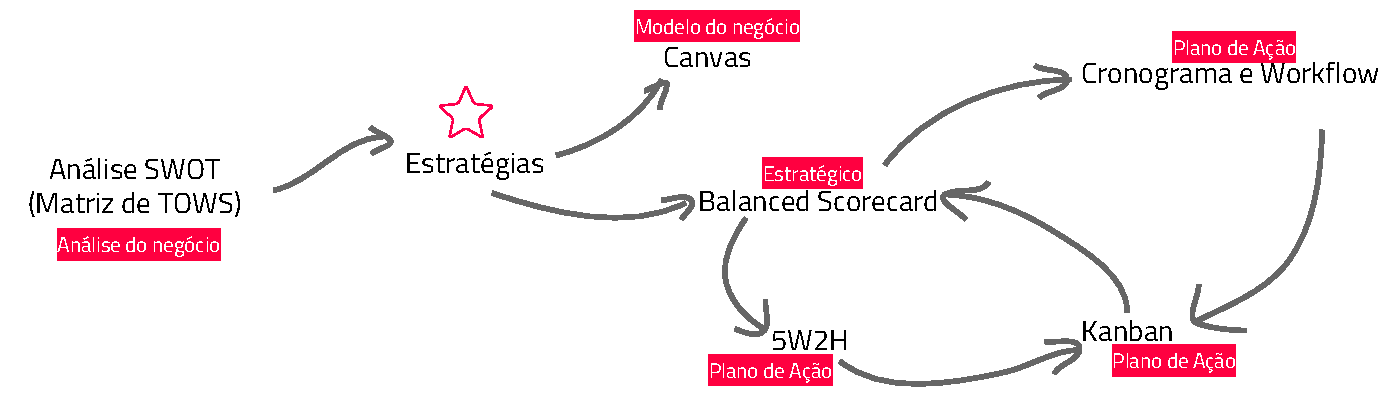
\includegraphics[width=\textwidth]{fluxograma_exemplo.pdf}
	\caption{Exemplo de fluxo de trabalho possível no sistema}
	\label{Rotulo}
\end{figure}

\section{Didática}

\section{Software (as a Service)}

\chapter{DESENVOLVIMENTO DO TRABALHO}

\section{Proposta e projeto do sistema}

\section{Desenvolvimento do projeto}

\chapter{RESULTADOS E DISCUSSÃO}

\chapter{CONCLUSÕES E TRABALHO FUTUROS}

\bibliography{teste}

\end{document}
